\chapter{Peaks für den Depolarisationsgrad}
\begin{figure}[h]
  \centering
  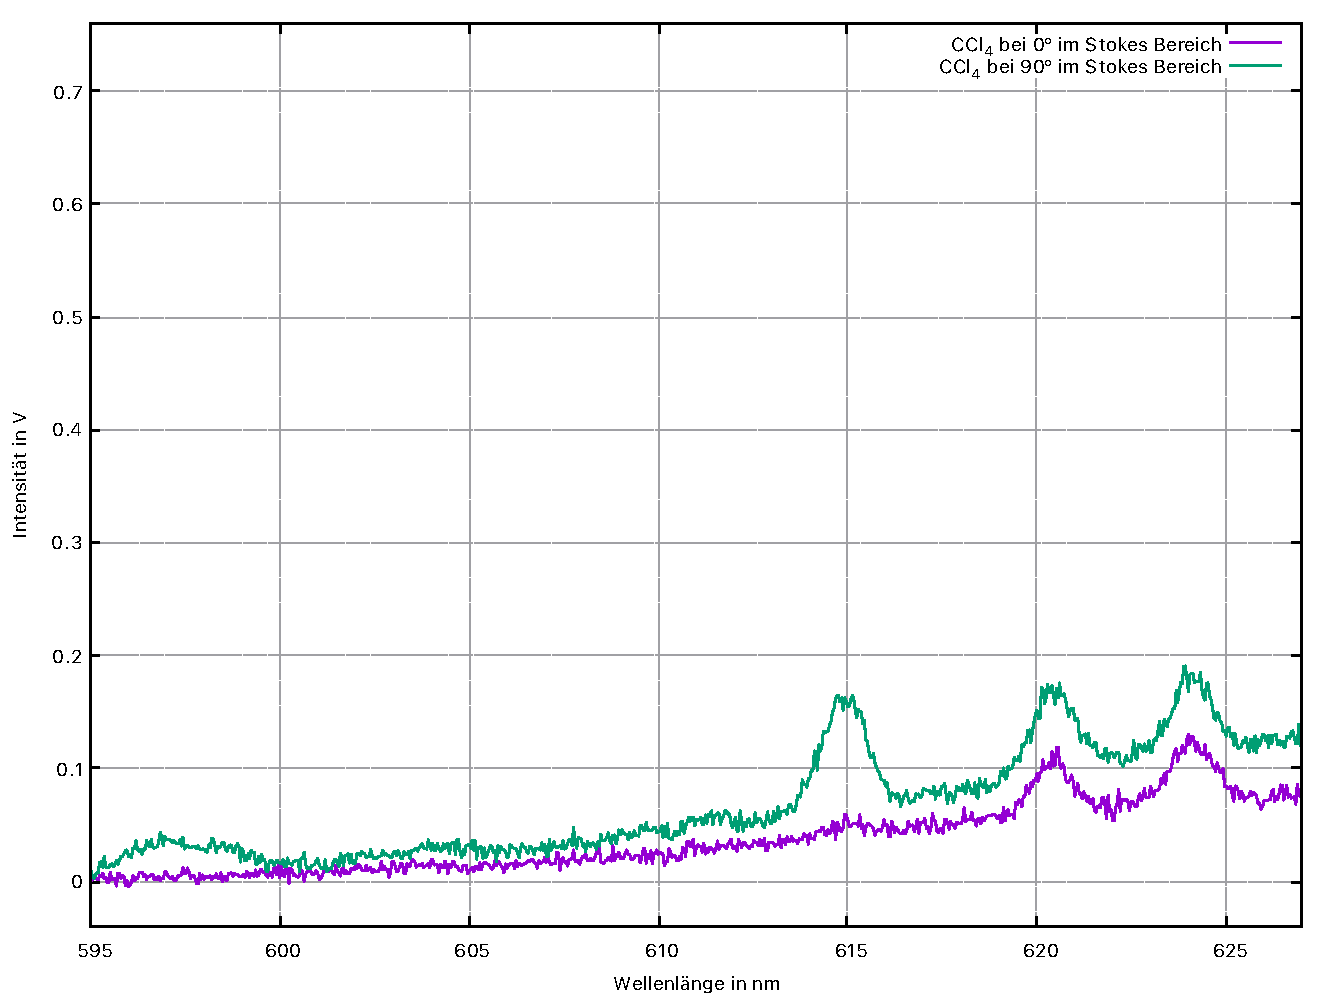
\includegraphics[scale=0.45]{Bilder/Verbesserung_Auswertung/ccl4_stokes.pdf}
  \caption{Spektrum von $CCl_4$, im Stokes Bereich bei 0° und 90° Polarisation.}
\end{figure}
\begin{figure}[h]
  \centering
  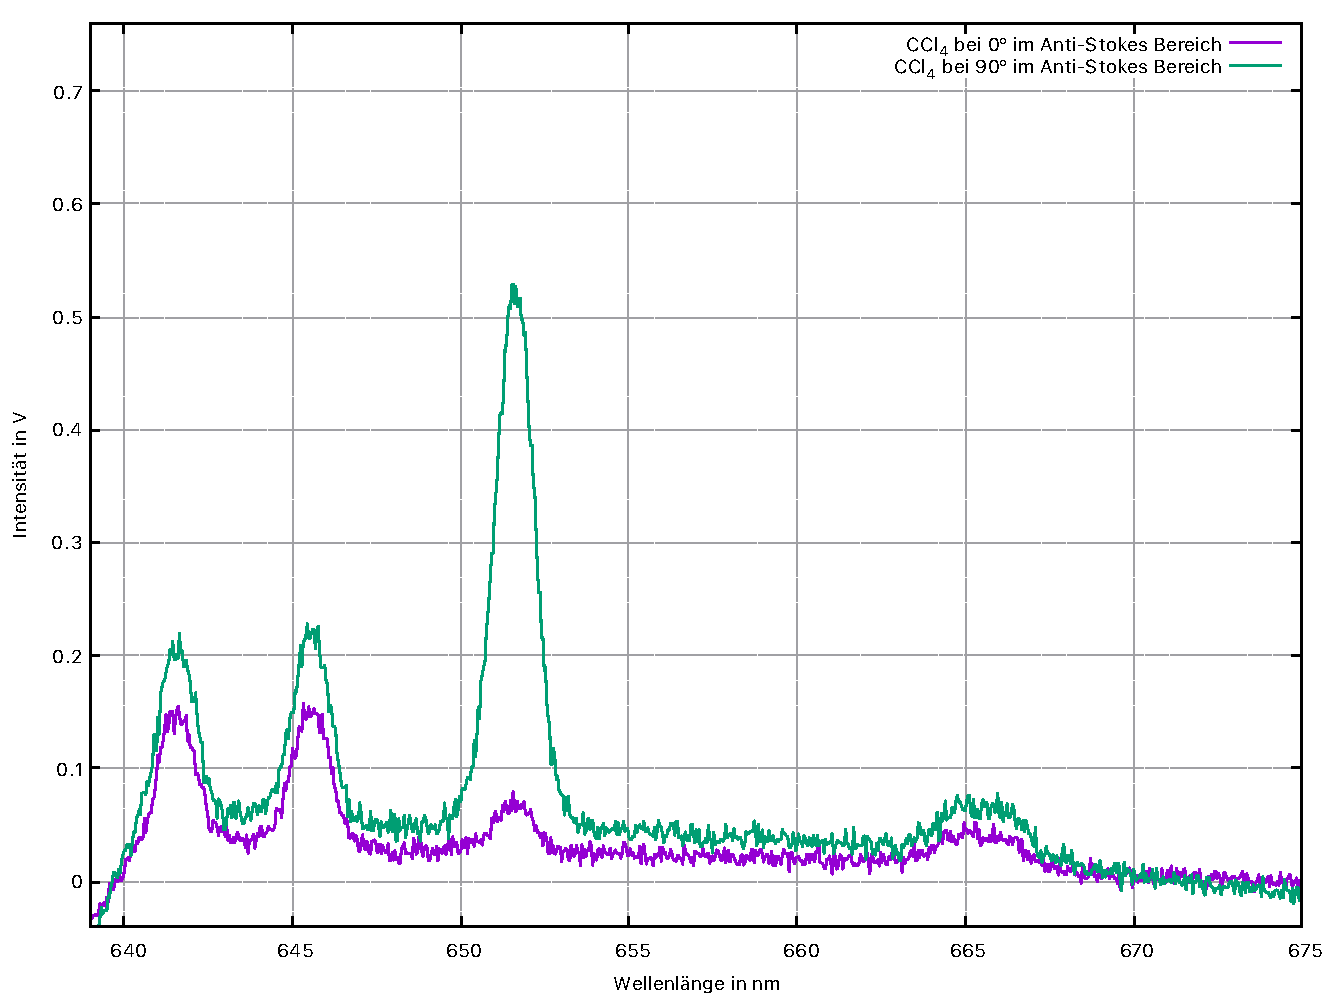
\includegraphics[scale=0.45]{Bilder/Verbesserung_Auswertung/ccl4_anti.pdf}
  \caption{Spektrum von $CCl_4$, im Anti-Stokes Bereich bei 0° und 90° Polarisation.}
\end{figure}
\begin{figure}[h]
  \centering
  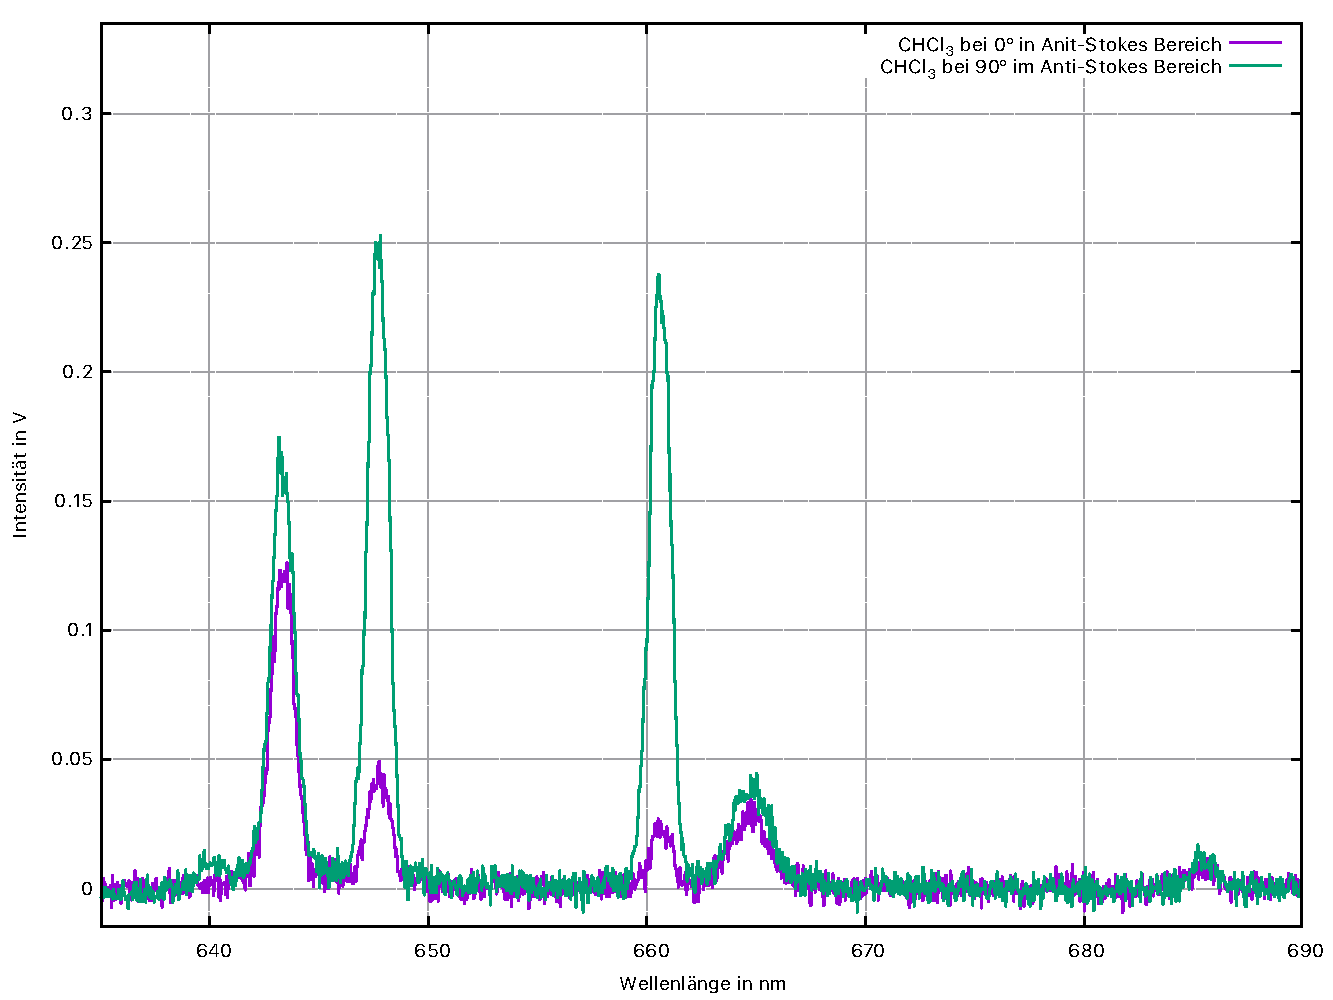
\includegraphics[scale=0.5]{Bilder/Verbesserung_Auswertung/chcl3_anti.pdf}
  \caption{Spektrum von $CHCl_3$, im Anti-Stokes Bereich bei 0° und 90° Polarisation.}
\end{figure}
\begin{figure}[h]
  \centering
  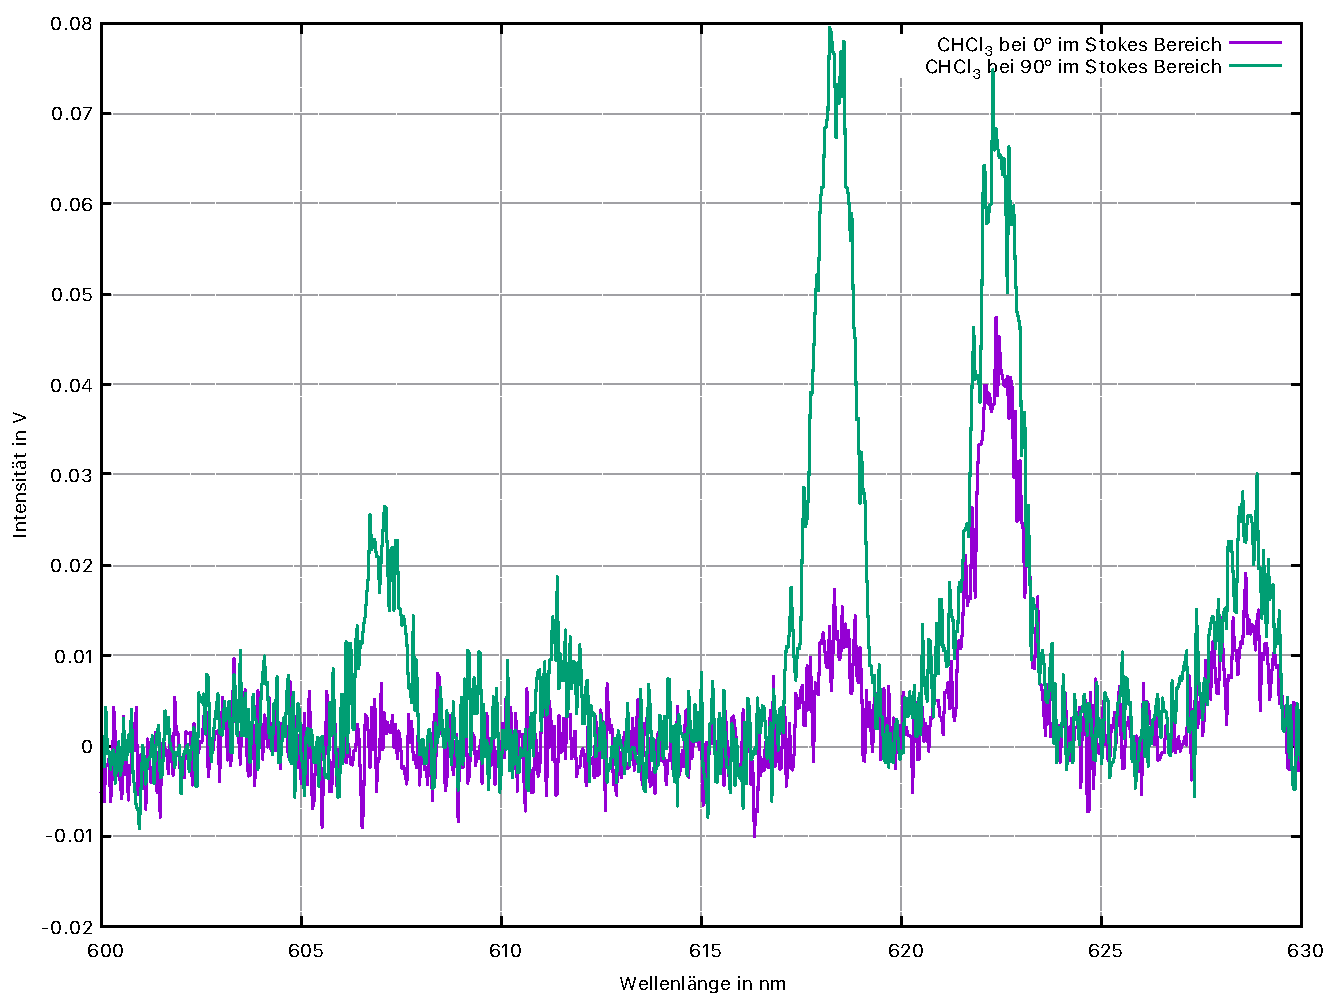
\includegraphics[scale=0.5]{Bilder/Verbesserung_Auswertung/chcl3_stokes.pdf}
  \caption{Spektrum von $CHCl_3$, im Stokes Bereich bei 0° und 90° Polarisation. In dem Bereich, indem es zur Überschneidung in der Wellenlänge bei den Peaks sowohl bei 0° als auch bei 90° kommt.}
\end{figure}

\chapter{Werte für Lage der Raman-Linien}
\begin{table}[h]
    \centering
    \begin{tabular}{c||c|c|c|c|c|c|c}
      \makecell{ $\lambda$ \\in nm} & $\nu$ in $\frac{1}{\text{cm}}$  & \makecell{ Fehler \\ $s_{\nu}$ in $\frac{1}{\text{cm}}$} & \makecell{Intensität\\ $0^{\circ}$ in V}  &  \makecell{Intensität\\ $90^{\circ}$ in V}  & \makecell{ Depolarisations- \\ grad $\rho$}  & \makecell{ Fehler \\ Depol. $s_{\rho}$} & Polarisation \\
      \hline
      643,3 & 270,4 & 12,1  & 0,1210 & 0,1688 & 0,7171 & 0,0365 & Depol. \\
      647,7 & 376,0 & 11,9  & 0,0470 & 0,2499 & 0,1879 & 0,0204 & Pol. \\
      660,7 & 679,8 & 11,5  & 0,0218 & 0,2279 & 0,0958 & 0,0220 & Pol. \\
      664,9 & 775,4 & 11,3  & 0,0281 & 0,0346 & 0,8123 & 0,1861 & Depol. \\
      685,3 & 1223,1 & 10,7  & 0,0088 & 0,0138 & 0,6359 & 0,4287 & Depol. \\  
    \end{tabular}
    \caption{Wellenlänge, Wellenzahl, Fehler der Wellenzahl, Intensität für 90° und 0°, Depolarisationsgrad und Fehler des Depolarisationsgrad für $CHCl_3$ im Anti-Stokes-Bereich.}
\end{table}
\begin{table}[h]
    \centering
    \begin{tabular}{c||c|c|c|c|c|c|c}
      \makecell{ $\lambda$ \\in nm} & $\nu$ in $\frac{1}{\text{cm}}$  & \makecell{ Fehler \\ $s_{\nu}$ in $\frac{1}{\text{cm}}$} & \makecell{Intensität\\ $0^{\circ}$ in V}  &  \makecell{Intensität\\ $90^{\circ}$ in V}  & \makecell{ Depolarisations- \\ grad $\rho$}  & \makecell{ Fehler \\ Depol. $s_{\rho}$} & Polarisation \\
    \hline
    643,3 & 270,4 & 12,1  & 0,1059 & 0,1747 & 0,6063 & 0,0335 & Depol. \\
    647,7 & 376,0 & 11,9  & 0,0434 & 0,2581 & 0,1681 & 0,0196 & Pol. \\
    659,9 & 661,5 & 11,5  & 0,0274 & 0,2651 & 0,1033 & 0,0190 & Pol. \\
    663,7 & 748,2 & 11,4  & 0,0320 & 0,0474 & 0,6754 & 0,1272 & Depol. \\
    671,4 & 921,0 & 11,1  & 0,0092 & 0,0181 & 0,5082 & 0,3092 & Depol. \\
  \end{tabular}%
\caption{Wellenlänge, Wellenzahl, Fehler der Wellenzahl, Intensität für 90° und 0°, Depolarisationsgrad und Fehler des Depolarisationsgrad für $CDCl_3$ im Anti-Stokes-Bereich.}
\end{table}\newpage
\begin{table}[h]
    \centering
    \begin{tabular}{c||c|c|c|c|c|c|c}
      \makecell{ $\lambda$ \\in nm} & $\nu$ in $\frac{1}{\text{cm}}$  & \makecell{ Fehler \\ $s_{\nu}$ in $\frac{1}{\text{cm}}$} & \makecell{Intensität\\ $0^{\circ}$ in V}  &  \makecell{Intensität\\ $90^{\circ}$ in V}  & \makecell{ Depolarisations- \\ grad $\rho$}  & \makecell{ Fehler \\ Depol. $s_{\rho}$} & Polarisation \\
      \hline
      639,0 & 165,8 & 12,3  & 0,0345 & 0,0655 & 0,5274 & 0,0863 & Depol. \\
      641,7 & 231,7 & 12,2  & 0,1201 & 0,7271 & 0,1652 & 0,0070 & Pol. \\
      655,1 & 550,4 & 11,7  & 0,0409 & 0,3626 & 0,1127 & 0,0139 & Pol. \\
      660,1 & 666,1 & 11,5  & 0,0841 & 0,1200 & 0,7007 & 0,0509 & Depol. \\  
    \end{tabular}%
    \caption{Wellenlänge, Wellenzahl, Fehler der Wellenzahl, Intensität für 90° und 0°, Depolarisationsgrad und Fehler des Depolarisationsgrad für $CHBr_3$ im Anti-Stokes-Bereich.}
\end{table}%
\begin{table}[h]
    \centering
    \begin{tabular}{c||c|c|c|c|c|c|c}
      \makecell{ $\lambda$ \\in nm} & $\nu$ in $\frac{1}{\text{cm}}$  & \makecell{ Fehler \\ $s_{\nu}$ in $\frac{1}{\text{cm}}$} & \makecell{Intensität\\ $0^{\circ}$ in V}  &  \makecell{Intensität\\ $90^{\circ}$ in V}  & \makecell{ Depolarisations- \\ grad $\rho$}  & \makecell{ Fehler \\ Depol. $s_{\rho}$} & Polarisation \\
      \hline
      641,5 & 226,8 & 12,2  & 0,1437 & 0,2009 & 0,7151 & 0,0306 & Depol. \\
      645,7 & 328,2 & 12,0  & 0,1472 & 0,2257 & 0,6520 & 0,0264 & Depol. \\
      651,7 & 470,8 & 11,8  & 0,0707 & 0,5163 & 0,1370 & 0,0098 & Pol. \\
      665,5 & 789,0 & 11,3  & 0,0381 & 0,0658 & 0,5793 & 0,0878 & Depol. \\  
    \end{tabular}
    \caption{Wellenlänge, Wellenzahl, Fehler der Wellenzahl, Intensität für 90° und 0°, Depolarisationsgrad und Fehler des Depolarisationsgrad für $CCl_4$ im Anti-Stokes-Bereich.}
  \end{table}%